\documentclass{article}
\usepackage{bigstrut}
\usepackage{adjustbox}
\usepackage{graphicx}^^M
\usepackage[T1]{fontenc}
\usepackage{float}
\usepackage{gensymb}
\usepackage{siunitx}
\usepackage{subfig}

\usepackage[english]{babel}
\usepackage[utf8]{inputenc}
\usepackage{indentfirst}

\addtolength{\oddsidemargin}{-.875in}
\addtolength{\evensidemargin}{-.875in}
\addtolength{\textwidth}{1.75in}
\addtolength{\textheight}{1in}

\begin{document}
\title{Design IV: Final Report}
\begin{titlepage}
    \centering
	{\scshape\LARGE Design IV: Final Report \par}
	\vspace{.5cm}
    {\scshape By:\par}
	{\scshape Richard Rossbach, MariaCristina Todaro, and Marcin Wisniowski \par}
	\vfill
	{\scshape Design IV, Weeks 10-14\par}
	\vspace{.5cm}
	{\scshape Stevens Institute of Technology\\E-232 Section LL Team 7\par}
	\vspace{.5cm}
	{\scshape supervised by\\Professor Lewis Natiello\par}
    \vfill
% Bottom of the page
	{\scshape“I pledge my honor that I have abided by the Stevens Honor System.”\par}
	\vspace{.5cm}
	{\scshape Richard Rossbach \hfill Date: 02/15/18\\MariaCristina	Todaro \hfill Date: 02/15/18\\Marcin Wisniowski \hfill Date: 02/15/18\\}
	\vspace{3cm}
\end{titlepage}

\tableofcontents
\newpage

\section{Introduction}
\indent The objective of this project is to design, implement, and test a filter and amplifier circuit that can optimize and equalize the performance of a speaker system consisting of a woofer and  midrange speakers. The team will be able to convert requirements into a feasible and optimal design by using  dynamic system modeling techniques and using methods for testing and characterization. Students hope to design a passive crossover network that separates a broadband signal into two signals which will then drive a speaker system. The design will be implemented through SimuLink before being built in order to create prototypes and circuit diagrams to work off of. The speaker system consists of a sub-woofer and a speaker appropriate for mid-range or high-frequency signals. The speaker/amplifier circuit will have a crossover frequency between 100-125 Hz and a filter slope of 12dB / octave or better. The group will be able to design an optimal crossover filter to split signals at the cutoff frequency and implement necessary power amplifiers so the sound output  can reach at least 75 db. Finally, students will be able to quantitatively demonstrate that the design requirements have been achieved.


\section{Material and Methods}
Before the group could begin designing and creating the circuit for the subwoofer, research was conducted in order to determine the best crossover filter to use as well as how a subwoofer operates. This was done so that the team could become familiar with the design task and the materials that would be used to complete the project. Of the four crossover filters that could be used (Butterworth, Chebyshev, Linkwitz-Riley, and Bessel), it was determined through research and analysis through our QFD (Table 1) that the Linkwitz-Riley crossover filter would be the best for the given project. The Linkwitz-Riley filter is a very popular filter choice for crossover networks. It is able to produce a -6 dB crossover point to achieve a maximally flat amplitude response. Furthermore, the summed group delay is flat. The group decided to create a second order system in order to minimize materials used, while also obtaining the correct minimum specifications. 

\begin{table}[h]
\begin{center}
\begin{tabular}{c|c|c|c|c}
& Butterworth & Chebyshev & Linkwitz-Riley & Bessel\\
\hline
Passband Accuracy & 10 & 4 & 6 & 9\\
\hline
Filter Slope & 7 & 10 & 5 & 6\\
\hline
Impulse Response & 5 & 7 & 10 & 3\\
\hline
Popularity in Crossover Filters & 3 & 3 & 7 & 3\\
\hline
Total & 25 & 24 & 28 & 21\\
\hline
Rank & 2 & 3 & 1 & 4\\
\end{tabular}
\caption{QFD}
\end{center}
\end{table}

When analyzing the QFD, it is clear that the Linkwitz-Riley filter is the best crossover filter to use for the crossover network. It will be able to have a crossover frequency between the required 100-125 Hz, will have a filter slope greater than 12 dB/octave, be able to be constructed with only passive components, and should be able to give an audio output greater than or equal to 75 dB. Although the other filter options may be able to do this as well, the team believes that the Linkwitz-Riley filter will be able to do fulfill these tasks the most efficiently and effectively.

\indent After determining the best filter for use in the circuit, the group used a spreadsheet to determine the optimal resistor values that would result in a gain of at least 75 dB. Using equations for voltage division, cutoff frequency, and current gain, the team was able to determine resistor values and capacitor values that would result in a gain of 75 dB:

\begin{center}
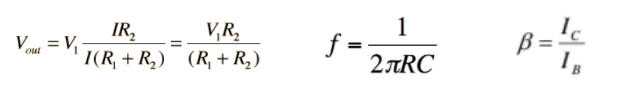
\includegraphics[width=400px]{Equations1.png}
\end{center}

After conducting these calculations, the group determined that the best resistors to use for a 75 dB gain would be $1750 \Omega$ for R2 and R3 and $3000 \Omega$ for R1 and R4. Proceeding with the project, the group went back to week 5 to design a circuit that could be used with the woofer. With the design requirements in mind, the following circuit was designed in Simulink (Figure 1):

\begin{figure}[h]
\begin{center}
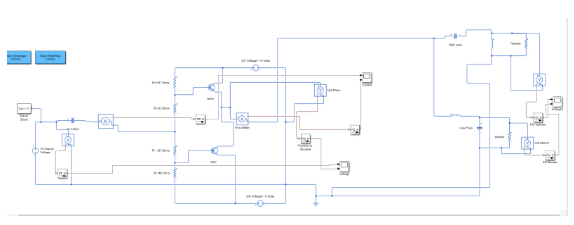
\includegraphics[width=\textwidth]{SimulinkCircuit.png}
\caption{Simulink Circuit}
\end{center}
\end{figure}

With resistor values of $1750 \Omega$ and $3000 \Omega$, capacitor values of $220 \mu F$ and inductor values of $10mH$, the circuit would be able to output the required gain and have the correct crossover frequency. These inductor and capactior values for the high pass and low pass crossover were determined using an online calculator (speakerwizard.co). Inputting the correct crossover frequency the group was able to find values for the inductors and capacitors that would make the crossover network work correctly. However, since these numbers were very specific, instead of putting multiple inductors in series and capacitors in parallel to get the exact values, the group decided to estimate nearby values that were readily available in supply. By using capacitor values of $220 \mu F$ and inductor values of $10mH$ the group was able to achieve a crossover frequency of 107 Hz, which was within project guidelines (between 100-125 Hz). 
\newpage

\begin{figure}[h]
\begin{center}
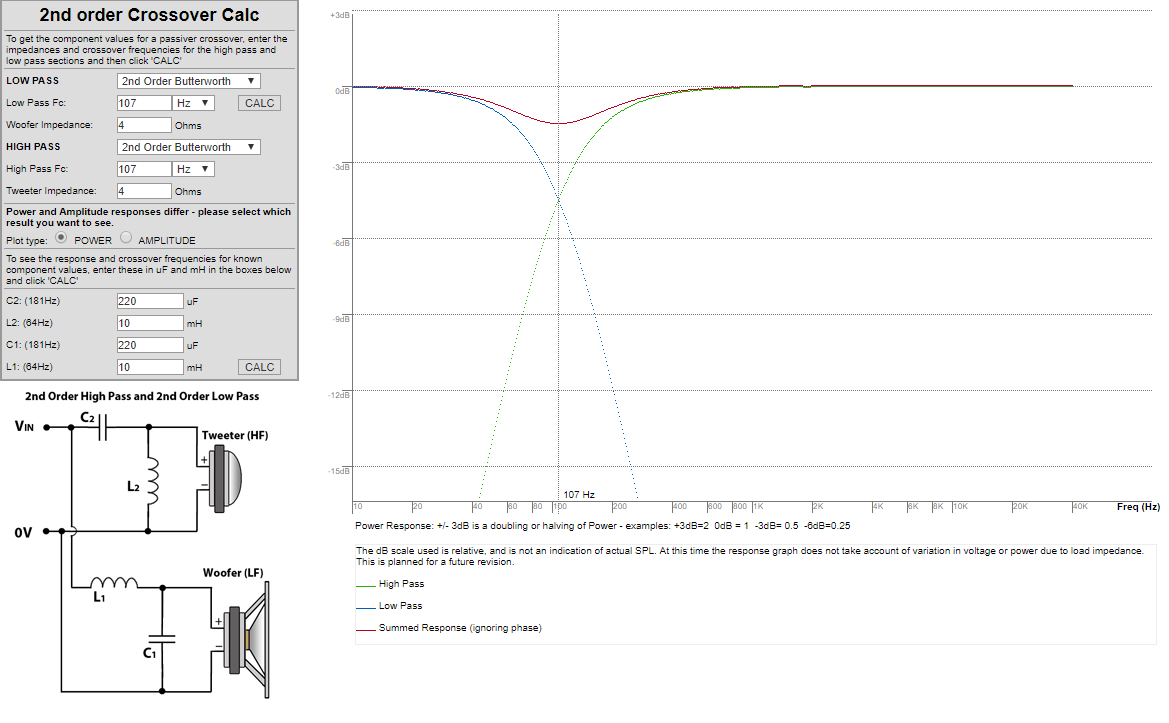
\includegraphics[width=\textwidth]{Crossover_Math.png}
\caption{Crossover Calculations}
\end{center}
\end{figure}


The following picture demonstrates the completed circuit connected to the speaker. The group was able to keep the circuit compact and color coded to easy navigation across different connections (Figures 3 and 4):
\newpage

\begin{figure}[h]
\begin{center}
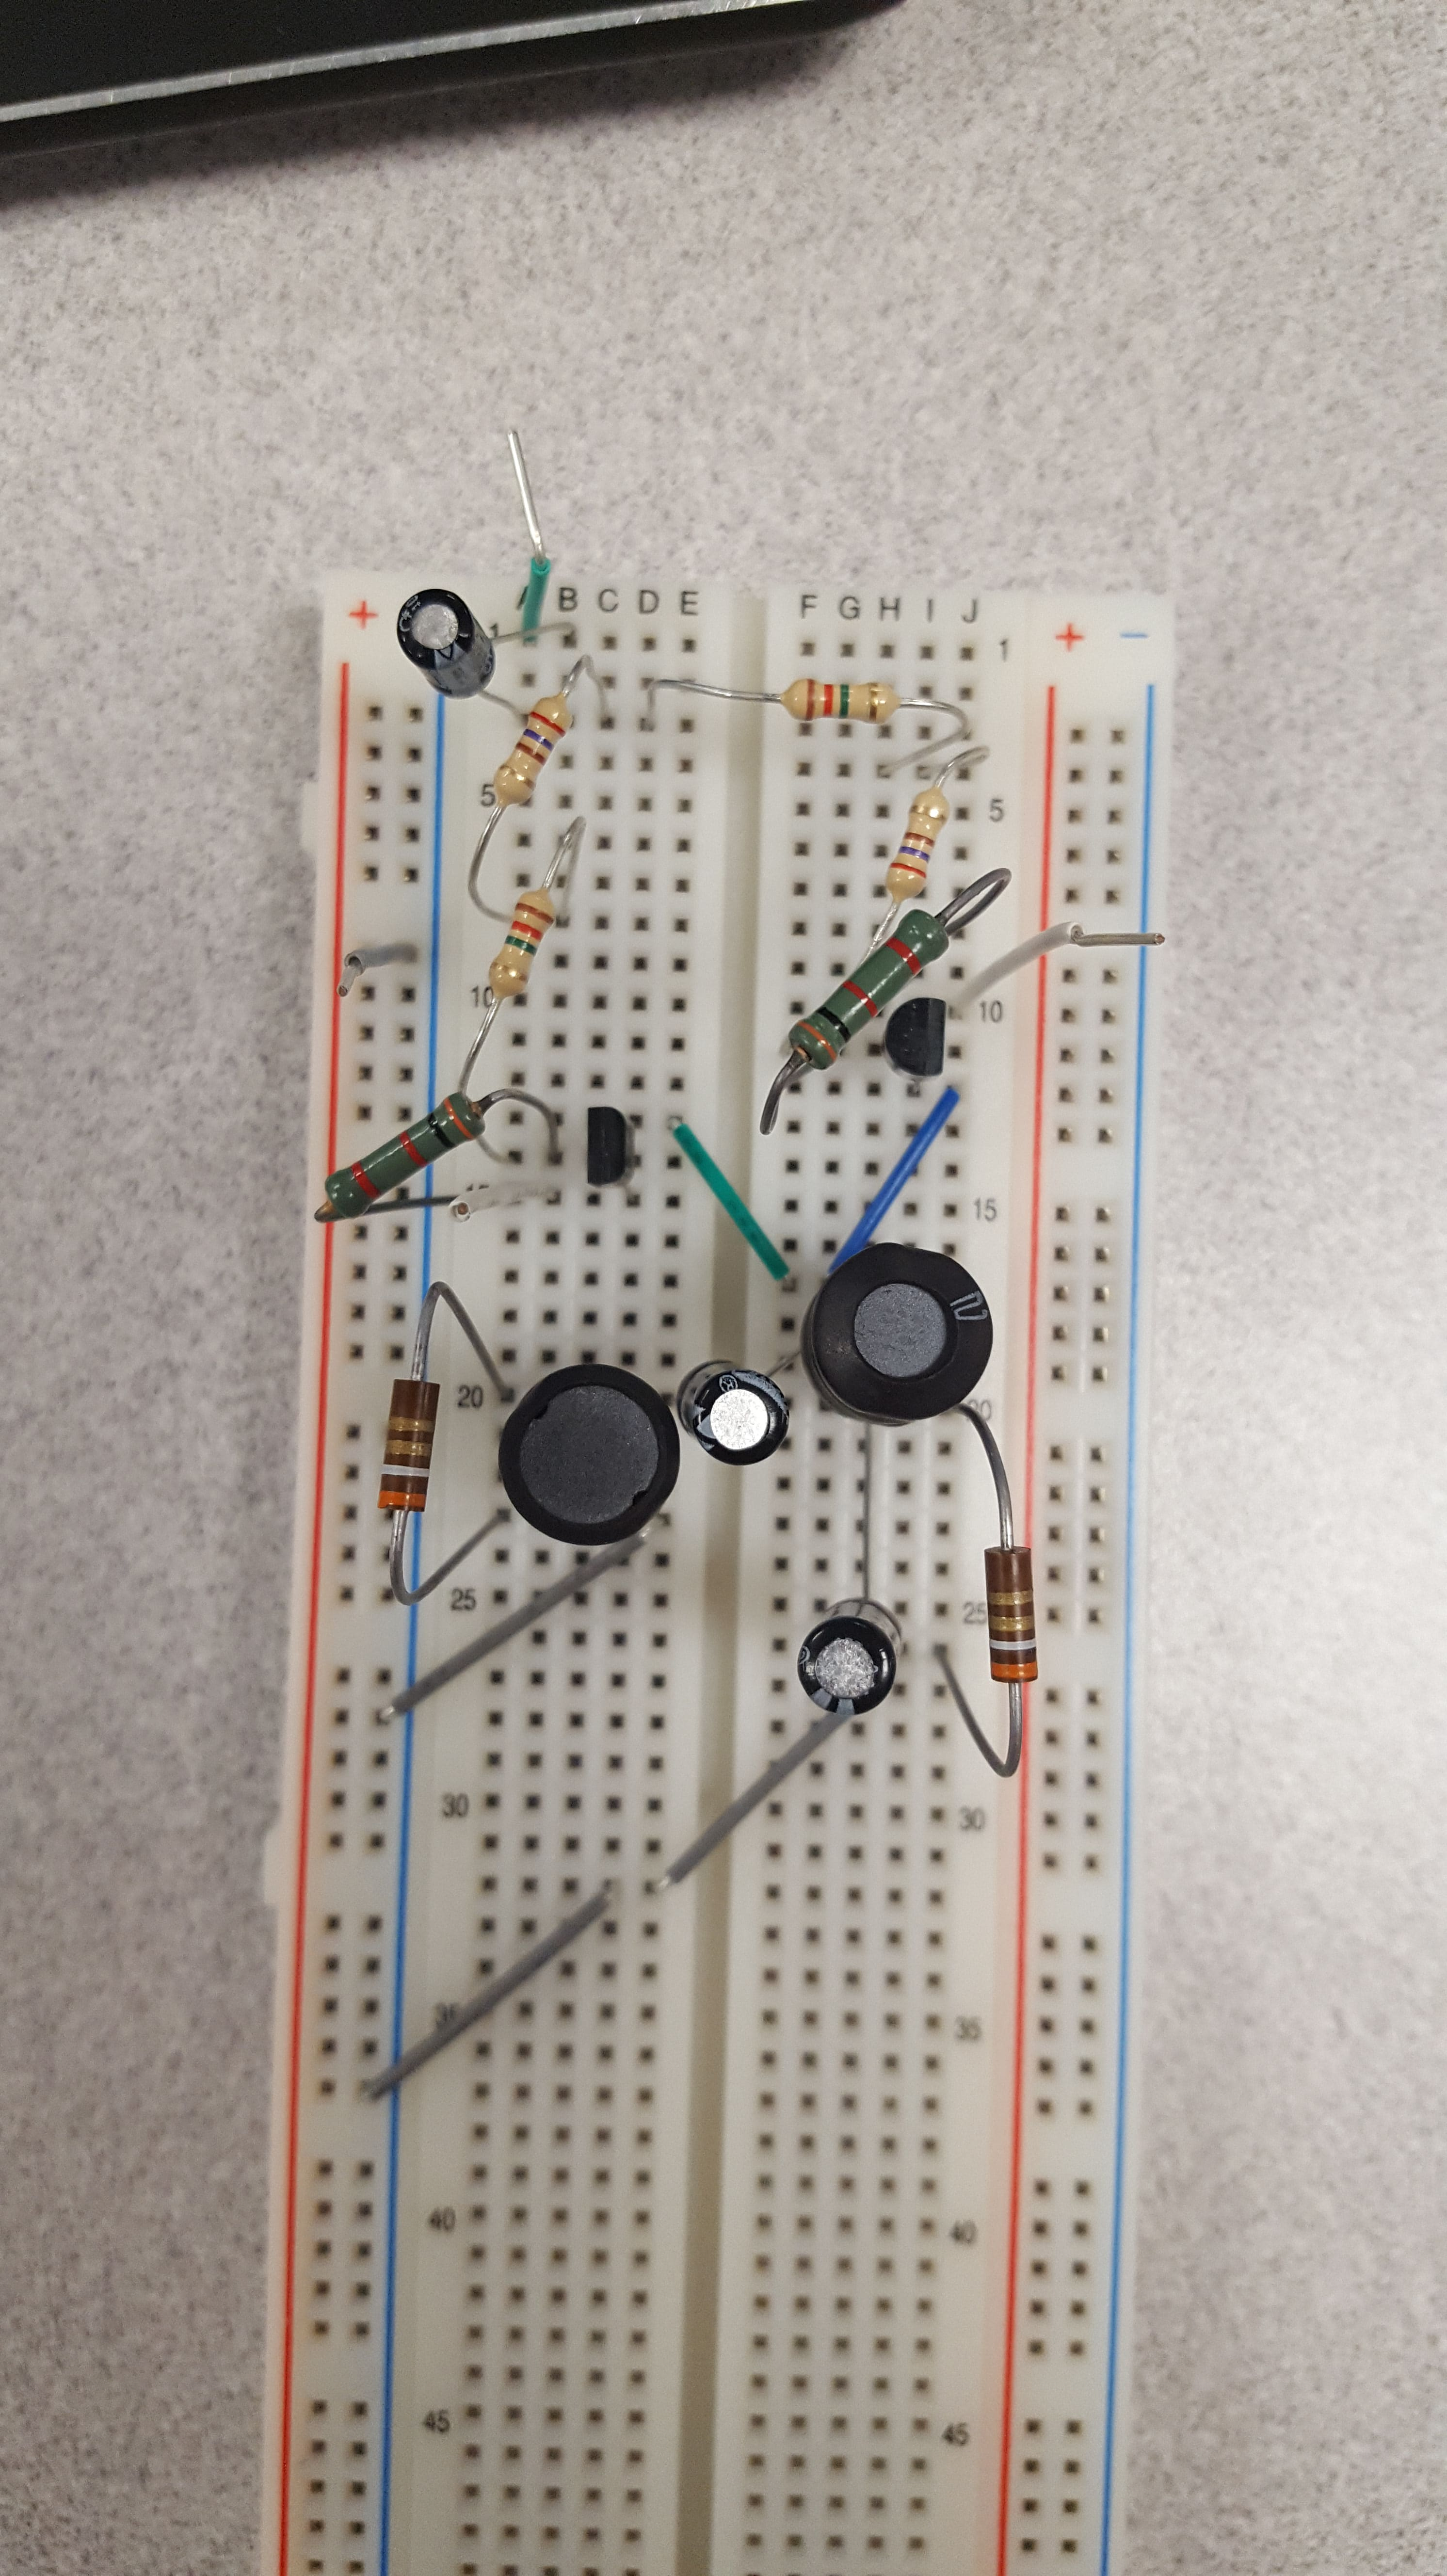
\includegraphics[width=200px]{DisconnectedCircuit-min.jpg}
\caption{Unconnected Circuit}
\end{center}
\end{figure}


\begin{figure}[h]
\begin{center}
\subfloat[Circuit Construction]{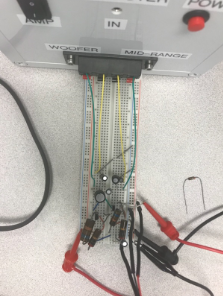
\includegraphics[width=5cm]{CircuitConstruction.png}}
\qquad \qquad \qquad
\subfloat[Circuit and Speaker]{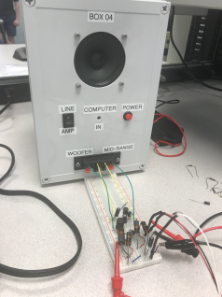
\includegraphics[width=5cm]{CircuitandSpeaker.png}}
\caption{Completed Circuit}
\end{center}
\end{figure}
\newpage

\section{Results}
After building our midrange woofer and sub woofer, the group tested its efficacy by measuring the output voltages at the low pass and high pass portions of the circuitry.

\begin{figure}[h]
\begin{center}
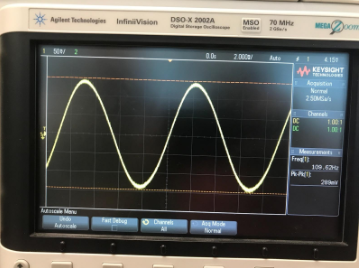
\includegraphics[width=250px]{LowPassFilterTest.png}
\caption{Low Pass Filter Test}
\end{center}
\end{figure}

As seen in Figure 5 with a input signal above the cutoff frequency, the circuit passed the low pass filter test because it had a peak-peak voltage that was a low voltage (289 mV). 
\newpage

\begin{figure}[h]
\begin{center}
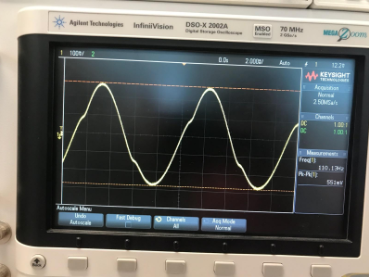
\includegraphics[width=250px]{HighPassFilterTest.png}
\caption{High Pass Filter Test}
\end{center}
\end{figure}

As seen in Figure 6 using the same frequency values, the circuit passed the high pass filter test because it had a peak-peak voltage that was a high voltage compared to that of the low pass (551 mV).   

\section{Discussion}
	Once the group built an effective circuit it was put through two tests.  The Low Pass and High Pass Filter Tests were conducted to compare the values of the voltages at different parts of the circuit and to see if our circuit could produce the frequencies necessary to produce quality sound from a speaker. The group also correlated the output frequencies of each filter. The output frequency of the high pass and low pass was the same at the cut off frequency proving that the circuit built was ready to be tested further using a speaker.  Once connected to the speaker, the group first tested sound by changing the frequency from very low to very high on the oscilloscope and this caused the sound to go from low pitched to high pitched, which means the low pass and high pass filters fed the correct voltages to the speaker and were not inverted in any way. The final test was then conducted which was to connect the speaker and circuit to a laptop to play music.  Once “My Way” by Frank Sinatra played on the speaker at a good volume, bass, and little static, the group could conclude that the midrange and sub woofer were designed and executed effectively. 
    
\indent There were some trials and errors before the group developed a successful circuit.  Originally, the group used resistor values of 3,000 and 1,750 to achieve a gain of 75 dB.  However, while the gain ratio was correct, not enough current was being supplied to the transistors to activate them.  This caused the circuit to short.  To combat the issue new calculations were done and the group decided to use resistor values of 20 and 160 instead.  This gave excellent sound and still allowed a gain of 75 dB. Furthermore, the group incorrectly wired up one of the transistors during one of the tests causing it to breakdown, so a new NPN transistor needed to be used. 

\subsection{Feedback}
\indent This project offered many opportunities for the team to learn about not only woofers but the circuitry and components that makes them up. The team learned more about the various components of a woofer like the amplifiers and transistors, as well as the components the group already had knowledge of such as the resistors and capacitors. Through the project the team was able to demonstrate a greater understanding for Simulink and how to use a Simulink model to develop a real working circuit. The project was given in a reasonable amount of time, with the group not feeling too pressured to finish nor feeling that too much time was given. Overall, the project was a great learning experience and the team recommends the project for future classes.


\setcounter{figure}{0}
\setcounter{table}{0}
\section{Appendix and References}
\begin{itemize}
\item https://jlaudio.zendesk.com/hc/en-us/articles/226655828-Setting-Crossovers-
\item https://www.audioholics.com/loudspeaker-design/filter-crossover-types-for-loudspeakers
\item http://www.speakerwizard.co.uk/calcs/Crossover\_Calc\_v2.php 
\end{itemize}

\subsection{Figures and Tables}

\begin{table}[h]
\begin{center}
\begin{tabular}{c|c|c|c|c}
& Butterworth & Chebyshev & Linkwitz-Riley & Bessel\\
\hline
Passband Accuracy & 10 & 4 & 6 & 9\\
\hline
Filter Slope & 7 & 10 & 5 & 6\\
\hline
Impulse Response & 5 & 7 & 10 & 3\\
\hline
Popularity in Crossover Filters & 3 & 3 & 7 & 3\\
\hline
Total & 25 & 24 & 28 & 21\\
\hline
Rank & 2 & 3 & 1 & 4\\
\end{tabular}
\caption{QFD}
\end{center}
\end{table}

\begin{figure}[h]
\begin{center}
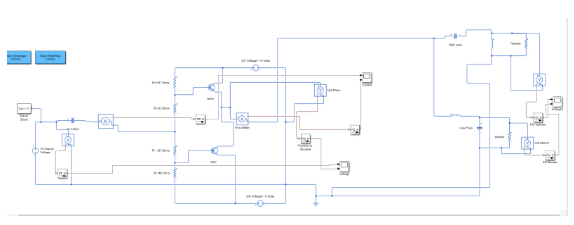
\includegraphics[width=\textwidth]{SimulinkCircuit.png}
\caption{Simulink Circuit}
\end{center}
\end{figure}

\begin{figure}[h]
\begin{center}
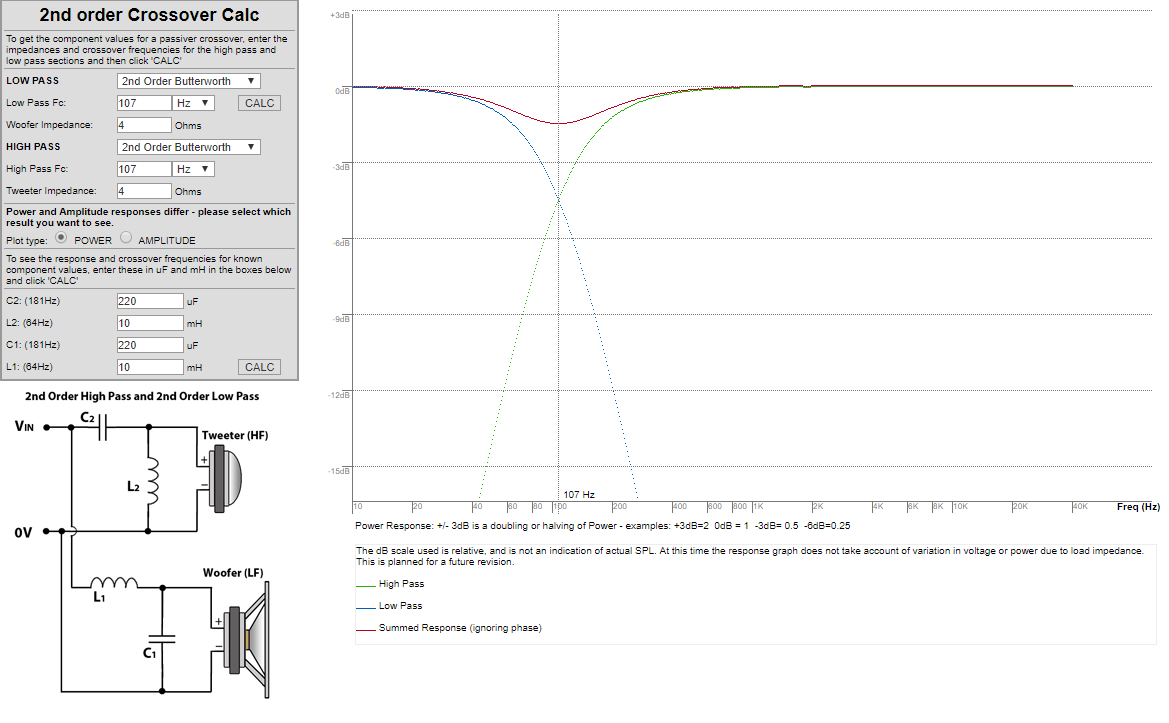
\includegraphics[width=\textwidth]{Crossover_Math.png}
\caption{Crossover Calculations}
\end{center}
\end{figure}

\begin{figure}[h]
\begin{center}
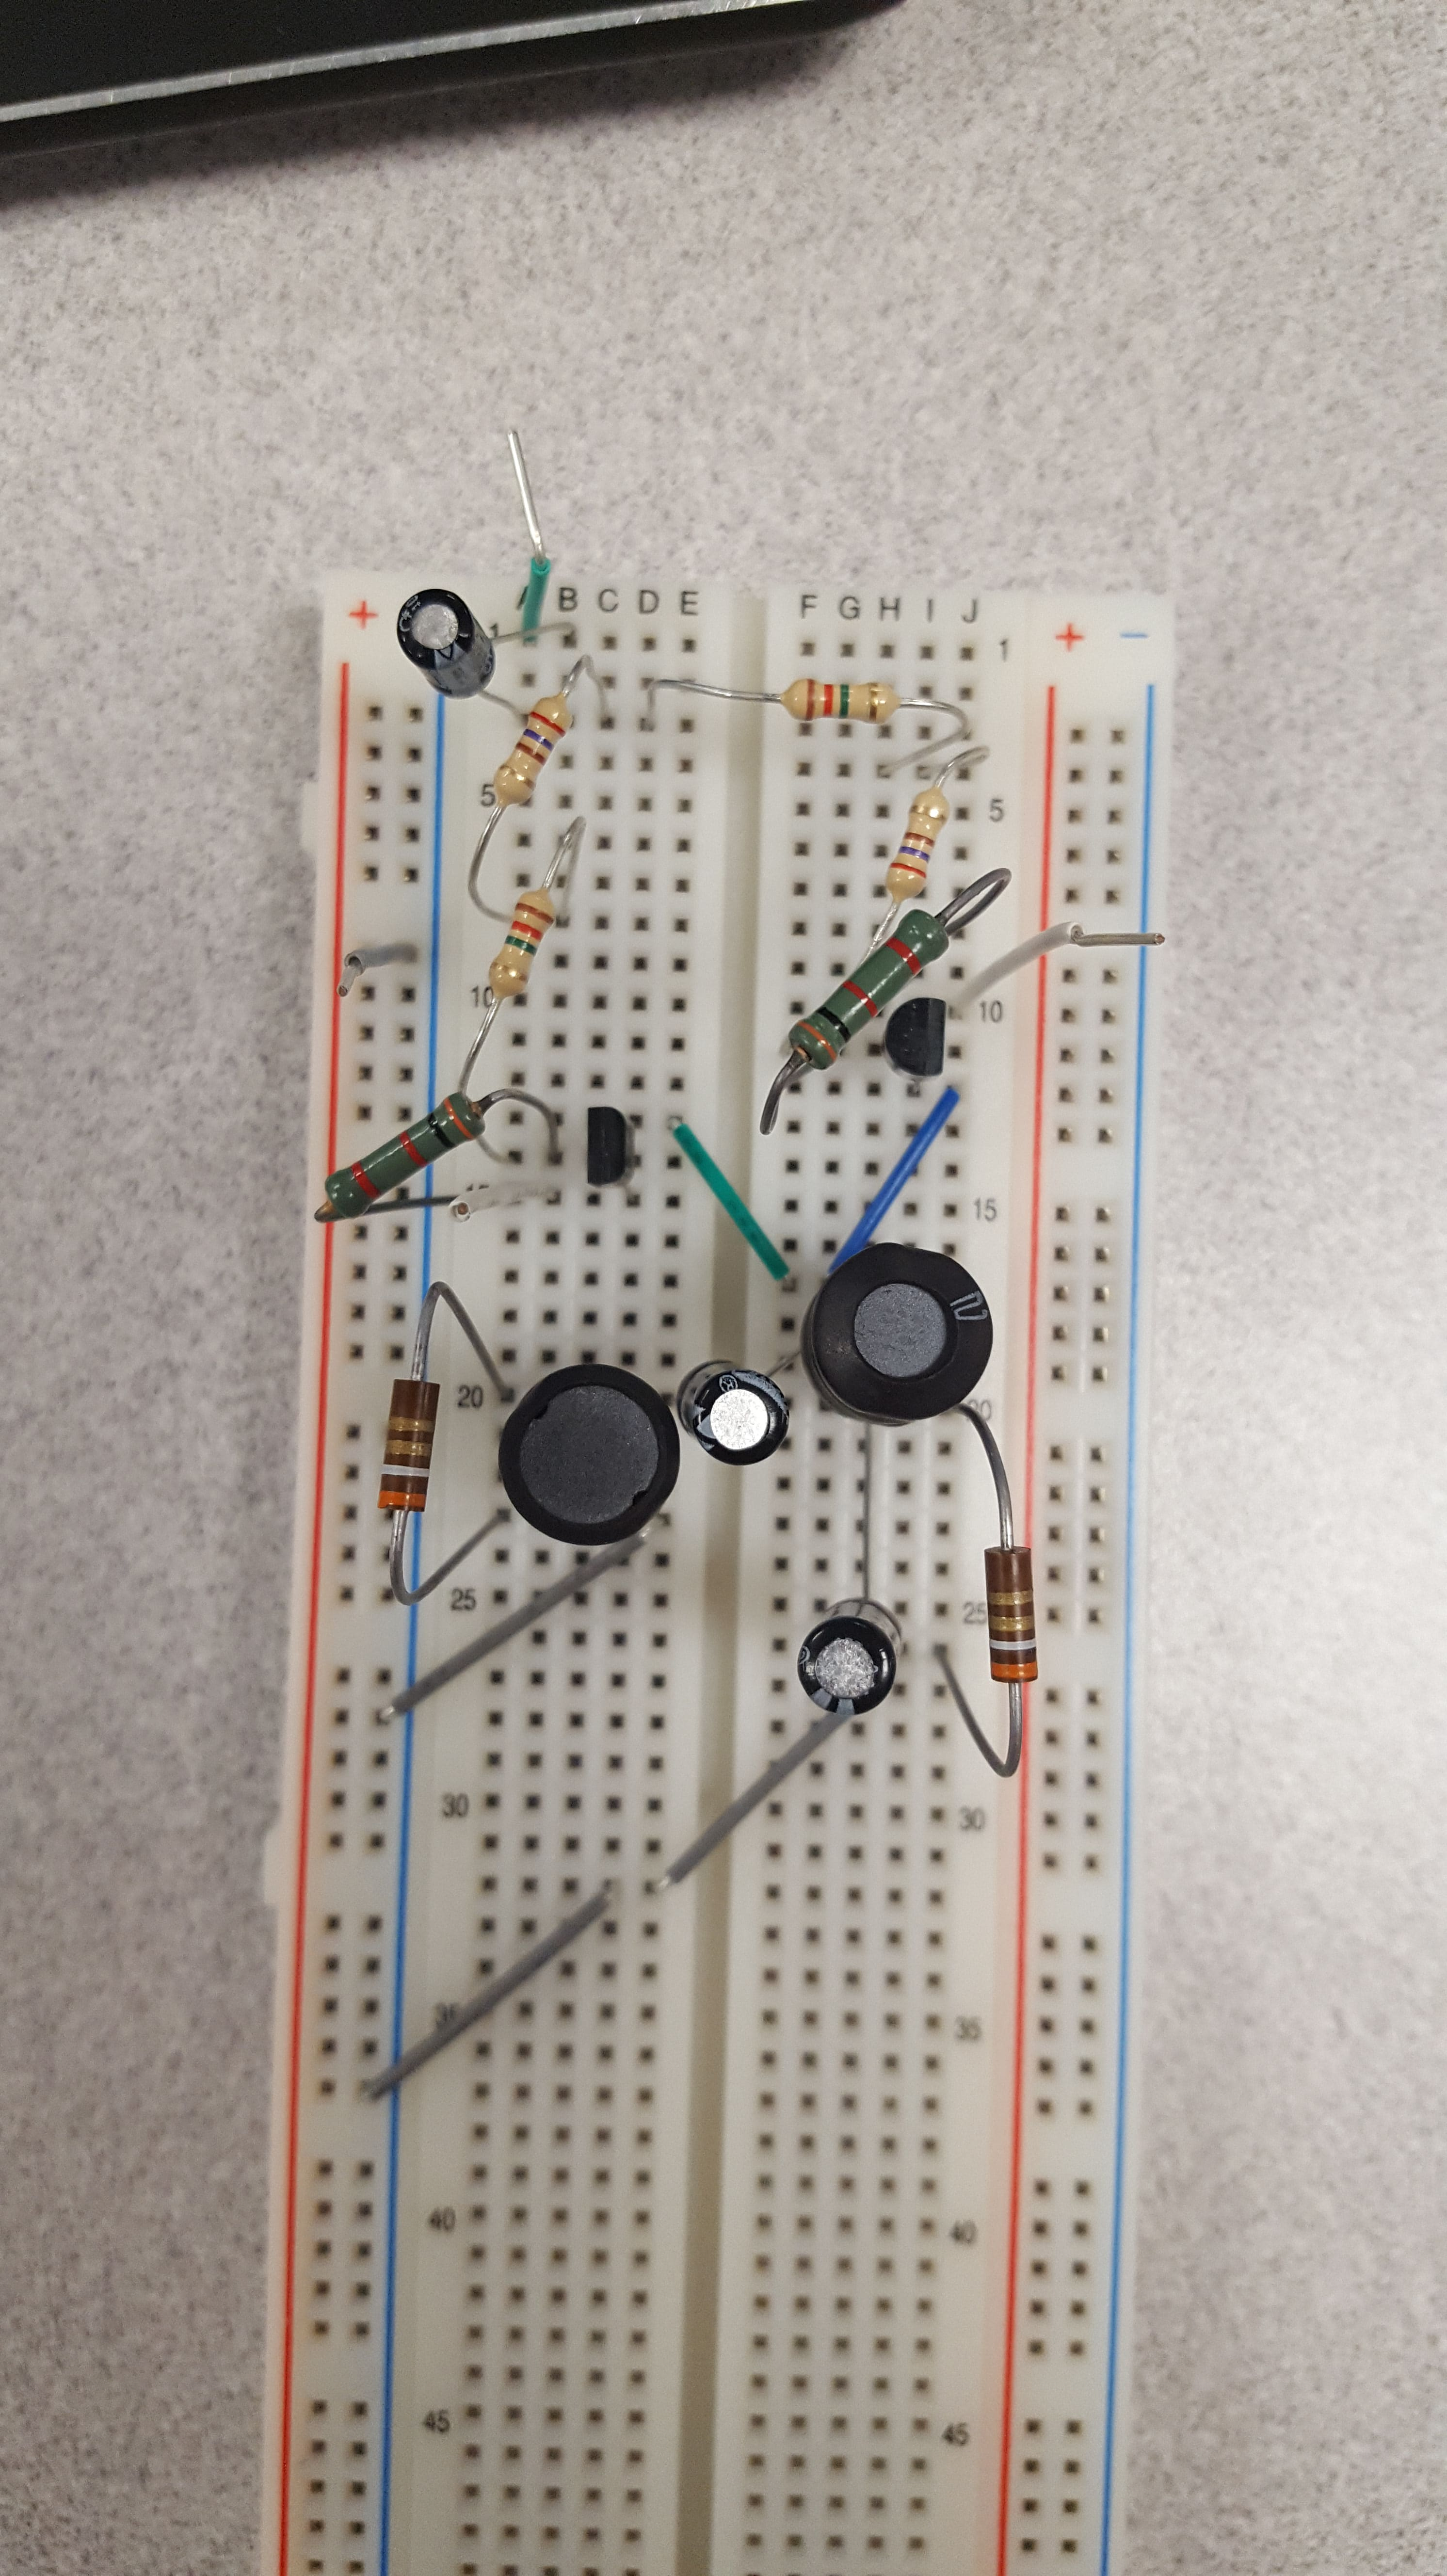
\includegraphics[width=200px]{DisconnectedCircuit-min.jpg}
\caption{Unconnected Circuit}
\end{center}
\end{figure}

\begin{figure}[h]
\begin{center}
\subfloat[Circuit Construction]{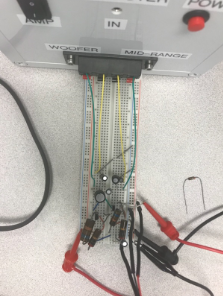
\includegraphics[width=5cm]{CircuitConstruction.png}}
\qquad \qquad \qquad
\subfloat[Circuit and Speaker]{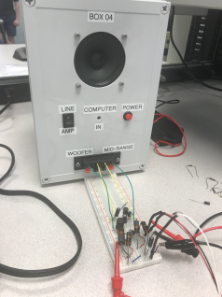
\includegraphics[width=5cm]{CircuitandSpeaker.png}}
\caption{Completed Circuit}
\end{center}
\end{figure}

\begin{figure}[h]
\begin{center}
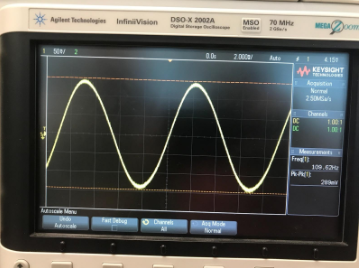
\includegraphics[width=250px]{LowPassFilterTest.png}
\caption{Low Pass Filter Test}
\end{center}
\end{figure}

\begin{figure}[h]
\begin{center}
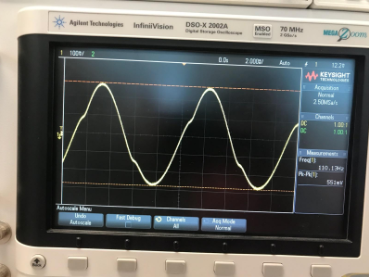
\includegraphics[width=250px]{HighPassFilterTest.png}
\caption{High Pass Filter Test}
\end{center}
\end{figure}

\end{document}